\chapter{Konfiguration}
\label{sec:konfig}

Um den Aufbau und die Einstellungen der grundlegenden Anwendung der Hoch\-schul-\ac{App} besser verstehen zu können, bietet es sich an, die Schritte, die bei der Erstellung dieser Anwendung durchgeführt worden sind, zu dokumentieren und zu erläutern. Im folgenden werden diese Schritte deshalb aufgeführt. Es soll jedoch nicht nur um die Einrichtung der Software im Allgemeinen gehen, sondern auch um die Einrichtung der Entwicklertools, die für die Arbeit an der Hochschul-\ac{App} bereitgestellt wurden.

\section{Entwicklungsumgebung}
\label{sec:entwicklungsumgebung}

Für die Arbeit am Prototypen der neuen Hochschul-\ac{App} wird das Nutzen einer \ac{IDE} empfohlen. Der Vorteil hierbei liegt in der Verwaltung der Projektstruktur, der Abhängigkeiten und der automatisierten Kompilierung des Quellcodes. Dabei ist es grundsätzlich egal, welche \ac{IDE} verwendet wird, da die meisten dieser Entwicklungsumgebungen die wichtigsten Funktionen bereits beinhalten. Dennoch wird hier explizit die Java \ac{IDE} \textit{IntelliJ IDEA} der Firma \textit{JetBrains} empfohlen\autocite[Siehe][]{intellij}. \textit{IntelliJ IDEA} wird in zwei Formaten angeboten, einer umfassenden \textit{Ultimate} Version, welche alle Funktionen der Anwendung beinhaltet, und einer vereinfachten \textit{Community} Edition, welche kostenfrei ist, jedoch nicht alle Features unterstützt. Studierende können sich kostenlos eine Lizenz für \textit{IntelliJ IDEA Ultimate} besorgen.\\
\linebreak
Im folgenden wird kurz die Einstellung der \ac{IDE} \textit{IntelliJ IDEA Ultimate} erläutert, welche nötig ist, um die Vorteile der geschaffenen Rahmenbedingungen vollständig zu nutzen. Die genutzte Version bei der Demonstration ist \textsc{IntelliJ IDEA 2019.3.1 (Ultimate Edition)}. Es wird hier noch einmal darauf hingewiesen, dass die Entwicklung unabhängig von der genutzten \ac{IDE} möglich ist, die Nutzung von \textit{Intellij IDEA} hier jedoch empfohlen wird. Außerdem soll hierbei auch noch einmal auf die Lizenzbedingungen der \textit{Ultimate} Version verwiesen werden\autocite[Siehe][]{ultimate}.

\subsection*{Hot Deploy}
\label{sec:hot_deploy}
       
\textit{Hot Deploy} ist eine Funktion, welche es ermöglicht, den Programmcode einer Software automatisiert bei der Erkennung von Änderungen oder beim manuellen Anstoßen einer Speicherung zu kompilieren und dann auf den laufenden Server zu deployen. Das erspart dem Entwickler die Wartezeit, die beim manuellen Deployment einer Serversoftware entsteht und ist bei der Entwicklerarbeit von großem Vorteil.

\subsubsection*{Einstellung in der \ac{IDE}}

Die Schritte zur Einrichtung sind folgende:

\begin{enumerate}

\item Öffnen der \ac{IDE} \textit{Intellij IDEA} und des Projektes, das die Microservices enthält
\item Öffnen des Menüpunktes \textit{File -> Settings} (Alternativ \textsc{STRG+ALT+S})
\item Auswählen der Option \textit{Build,Execution,Deployment -> Compiler}

\begin{figure}[H]
\centering
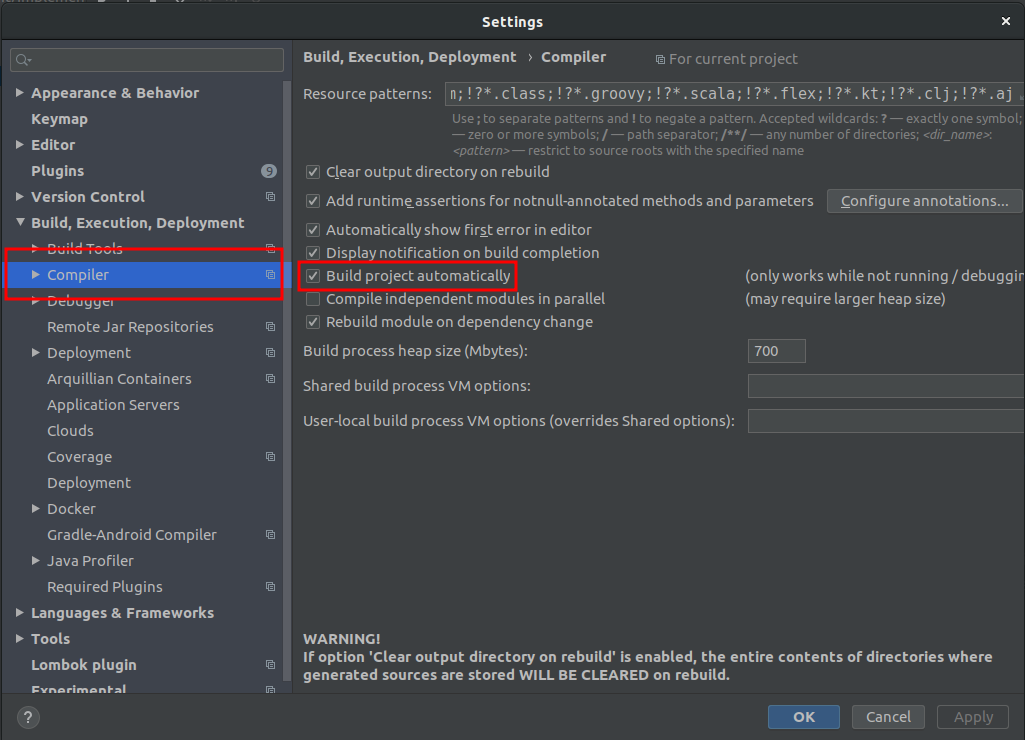
\includegraphics[width=\pictureWidth cm]{Bilder/Kapitel_4/hotdeploy.png}
\caption{Hot Deployment in \textit{IntelliJ}\label{fig:hotdeploy}}
\end{figure}

\item Bestätigen der Checkbox \textit{Build project automatically}

\item Öffnen der \textit{Registry} 

\begin{enumerate}

\item Tastenkombination \textsc{STRG+N}
\item Erweitern des Suchradius auf \textit{All}
\item Suchen nach Registry
\item Auswählen des Punktes \textit{Actions -> Registry...}
\begin{figure}[H]
\centering
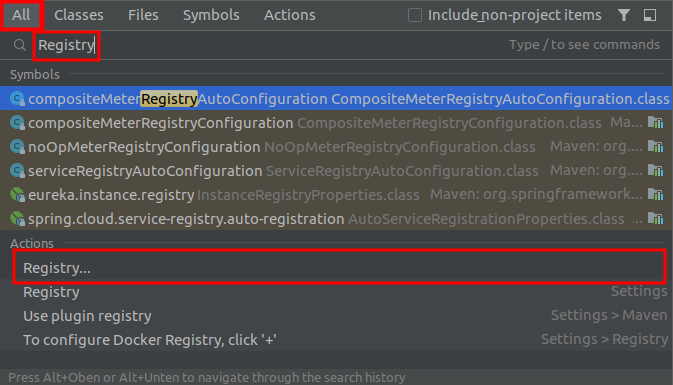
\includegraphics[width=\pictureWidth cm]{Bilder/Kapitel_4/registry.png}
\caption{Öffnen der Registry in \textit{IntelliJ}\label{fig:registry}}
\end{figure}

\end{enumerate}

\item Bestätigen der Checkbox \textit{compiler.automake.allow.when.app.running}

\begin{figure}[H]
\centering
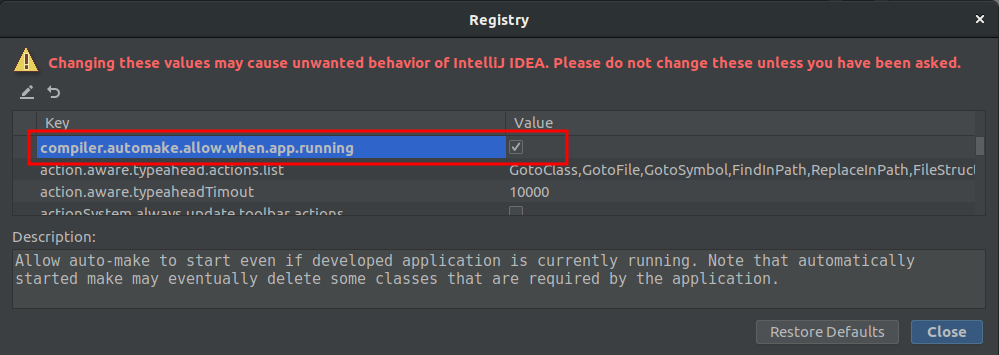
\includegraphics[width=\pictureWidth cm]{Bilder/Kapitel_4/compiler_hotdeploy.png}
\caption{Compiler Anweisung in \textit{IntelliJ}\label{fig:compiler_hotdeploy}}
\end{figure}

\item Neustart der \ac{IDE}

\end{enumerate}

Der Start der Services erfolgt nach wie vor manuell. Sobald der Service läuft, werden Änderungen automatisch in den laufenden Server übernommen.

\begin{figure}[H]
\centering

\includegraphics[width=\pictureWidth cm]{Bilder/Kapitel_4/start.png}
\caption{Start des Services in \textit{IntelliJ}\label{fig:start}}
\end{figure}

Hierbei startet der \textit{Play}-Button den Service normal, während der Button mit dem Käfer als Icon den Service im \textit{Debug}-Modus startet.

\subsubsection*{Manuelles Deployment}

Das \textit{Hot Deployment} wird in der Regel bei der Erkennung von Änderungen und in der \ac{IDE} \textit{IntelliJ IDEA} beim Drücken der Tastenkombination \textsc{STRG+S} angestoßen. Das kann auch der Fall sein, wenn gerade erst am Code geschrieben wird und die Software noch nicht kompilierbar ist. Außerdem verbraucht diese Funktion deutlich mehr Ressourcen auf dem \ac{PC} des Entwicklers, was es zu einer Funktion macht, die eventuell nicht gewünscht ist. In diesem Fall kann ein Service der Hochschul-\ac{App} folgendermaßen manuell deployed werden:

\begin{enumerate}

\item Start des Services wie in automatischem Deployment
\item Neustart des Services über Toolbar

\begin{figure}[H]
\centering
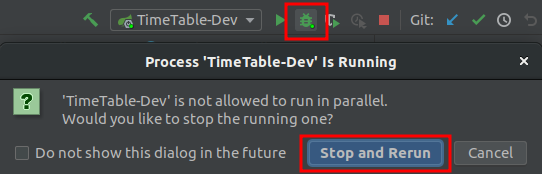
\includegraphics[width=\pictureWidth cm]{Bilder/Kapitel_4/rerun.png}
\caption{Neustart des Services in \textit{IntelliJ}\label{fig:rerun}}
\end{figure}

\end{enumerate}


\subsection*{Lombok}
\label{sec:lombok}

\textit{Lombok} ist ein Framework, welches es ermöglicht, einfachen Code, der sich in jedem \ac{POJO} befindet, nicht immer wieder neu tippen zu müssen. Durch einfache Annotations können so den \acp{POJO} \textit{Getter}, \textit{Setter}, \textit{Konstruktoren} und andere häufig verwendeten Codeabschnitte zur Kompilierzeit hinzugefügt werden. Das macht das manuelle Erstellen dieser Codeabschnitte überflüssig und macht das Projekt allgemein lesbarer, da durch die Annotations die eigentlichen Methoden-Implementierungen entfallen\autocite[][]{lombok}. Ein solches \ac{POJO} könnte nach der Nutzung von \textit{Lombok} folgendermaßen aussehen:
\newpage

\begin{lstlisting}[caption={Klassendefinition mit \textit{Lombok}}]
package test.lombok.pojo

import lombok.AllArgsConstructor;
import lombok.Getter;
import lombok.Setter;

@Getter
@Setter
@AllArgsConstructor
class POJO {
	private int attr1;
	private int attr2;    
}
\end{lstlisting}

\textit{Lombok} wird im Sourcecode des Prototypen der neuen Hochschul-\ac{App} bereits verwendet und sollte so auch in der \ac{IDE} der Entwickler konfiguriert werden, da diese sonst möglicherweise den verwendeten Sourcecode nicht kompiliert, da sie nicht erkennt, dass verwendete Methodenreferenzen von \textit{Lombok} erst zur Kompilierzeit hinzugefügt werden. Die Konfiguration in \textit{IntelliJ IDEA} erfolgt folgendermaßen:

\begin{enumerate}

\item Öffnen der \ac{IDE} \textit{Intellij IDEA} und des Projektes, das die Microservices enthält
\item Öffnen des Menüpunktes \textit{File -> Settings} (Alternativ \textsc{STRG+ALT+S})
\item Auswählen der Option \textit{Plugins}
\item Suche nach dem Plugin \textit{Lombok}

\begin{figure}[H]
\centering
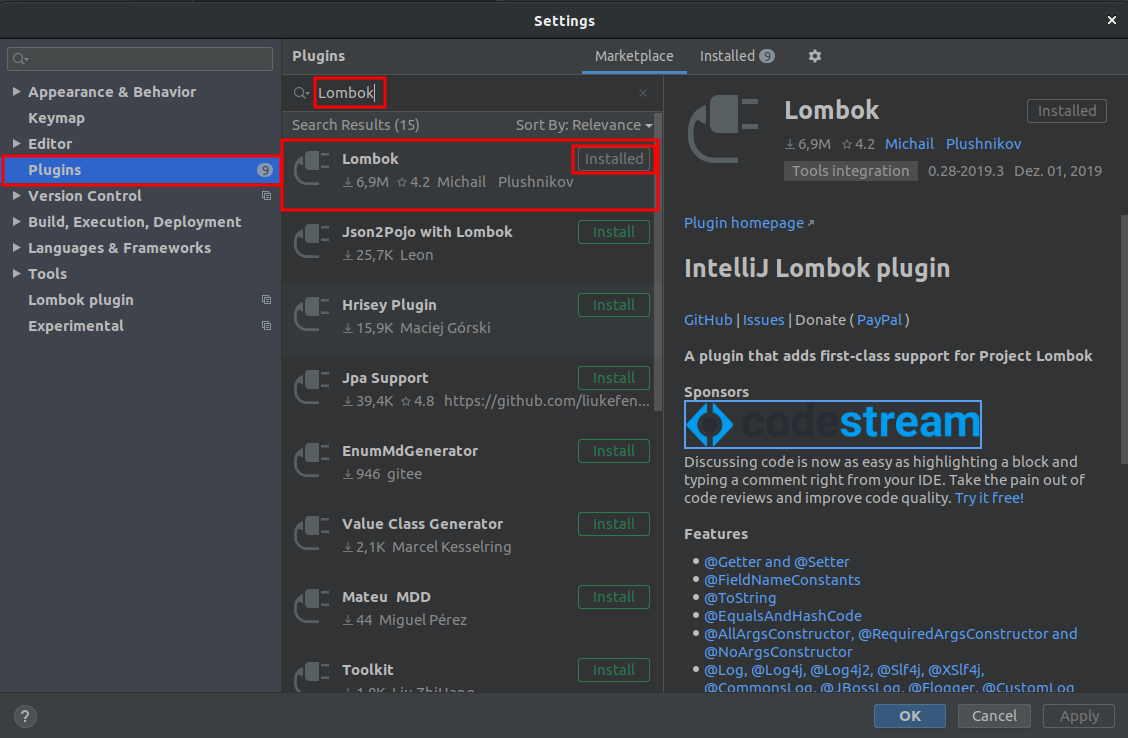
\includegraphics[width=\pictureWidth cm]{Bilder/Kapitel_4/lombok_plugin.png}
\caption{Lombok Plugin in \textit{IntelliJ}\label{fig:lombok_plugin}}
\end{figure}

\item Installation des Plugins und Neustart der \ac{IDE}

\end{enumerate}

\section{Spring Boot}
Wie bereits in Kapitel \ref{sec:framework} erwähnt wurde, wird \textit{Spring Boot} als Microservice Framework für den Prototypen der neuen Hochschul-\ac{App} verwendet. \textit{Spring} ist ein Framework, das durch die vereinfachte Einbindung anderer Bibliotheken die Entwicklung mit Java deutlich vereinfacht\autocite[Vgl.][1]{spring}. \textit{Spring Boot} zeichnet sich vor allem dadurch aus, dass es Elemente aus dem Java \ac{EE} Umfeld sowie open-source Bibliotheken zur Server-Entwicklung mit Fokus auf Microservices vereint. Im folgenden soll nun auf die Einbindung des \textit{Spring Boot} Frameworks in das Gesamtprojekt eingegangen werden.

\subsection*{Spring Initalizr}

\textit{Spring Initializr} ist ein Dienst der Entwickler des \textit{Spring} Frameworks, mit dem man voreingestellte Projekte erstellen und aus dem Dienst herunterladen kann. Dabei gibt man lediglich an, welche Abhängigkeiten das neue Projekt benötigt und mit welchen Versionen der Abhängigkeiten und Programmiersprachen das Projekt laufen soll. Durch diesen Dienst wurde ebenfalls der Prototyp der neuen Hochschul-\ac{App} erstellt, wobei hier zu beachten ist, dass alle Microservices als einzelnes Projekt betrachtet werden müssen und deshalb jeder Service seine eigenen Abhängigkeiten besitzt. Im folgenden wird kurz die Vorgehensweise zum Erstellen des Projektes erläutert, danach werden dann die einzelnen Abhängigkeiten aufgelistet.

\subsubsection*{Erstellen des Projekts}

Um ein Projekt mit \textit{Spring Initializr} zu erstellen, muss man die Website \textit{https://\-start.spring.io/} aufrufen. Danach durchläuft man folgende Schritte. Alle Abbildungen in der folgenden Abbildung stammen von der Website des Dienstes\autocite[][]{initializr}.

\begin{enumerate}

\item \textbf{Auswahl des Projekt Build Tools und Dependency Managements}\\
Für dieses Projekt wurde \textit{Maven} ausgewählt. Mehr Informationen dazu sind in Kapitel \ref{sec:build_tool} zu finden.
\begin{figure}[H]
\centering

\includegraphics[width=\pictureWidth cm]{Bilder/Kapitel_4/init_project.png}
\caption{Projektwahl in \textit{Spring Initializr}\label{fig:init_project}}
\end{figure}

\item \textbf{Wahl der Programmiersprache}\\
\textit{Spring Boot} unterstützt aktuell Java, Kotlin und Groovy. Für dieses Projekt wurde Java gewählt, zu diesem Thema wurde eine ausführliche Analyse in Kapitel \ref{sec:programmiersprache} angefertigt.
\begin{figure}[H]
\centering

\includegraphics[width=\pictureWidth cm]{Bilder/Kapitel_4/init_sprache.png}
\caption{Programmiersprachenwahl in \textit{Spring Initializr}\label{fig:init_sprache}}
\end{figure}

\item \textbf{Wahl der \textit{Spring Boot} Version}\\
Bei der Wahl der Version des Frameworks sollte man grundsätzlich eine Version wählen, die bereits aus der Snapshot Phase heraus ist. So umgeht man unvorhergesehene Fehler.
\begin{figure}[H]
\centering
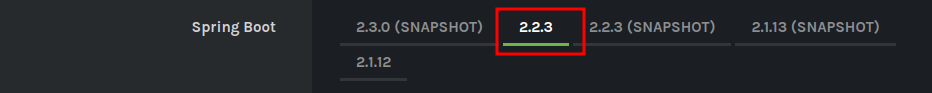
\includegraphics[width=\pictureWidth cm]{Bilder/Kapitel_4/init_version.png}
\caption{Versionswahl in \textit{Spring Initializr}\label{fig:init_version}}
\end{figure}

\item \textbf{Einstellung der Projekt Metadaten}\\
\textit{Maven} Projekte erfordern der Eingabe einiger Projekt-Metadaten. Darunter fallen die \textit{Group}, welche die Organisationseinheit beschreiben soll, welche das Projekt implementiert, diverse Bezeichner für das Projekt an sich und die Version der Programmiersprache, mit der das Projekt implementiert werden soll. 
\begin{figure}[H]
\centering
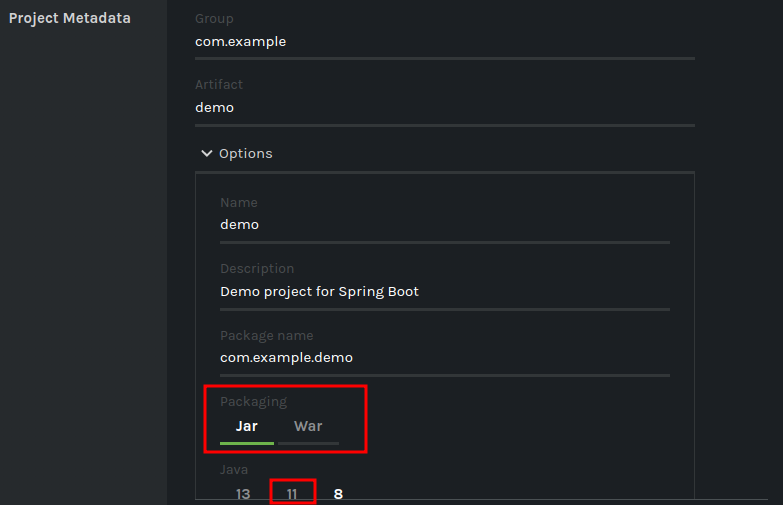
\includegraphics[width=\pictureWidth cm]{Bilder/Kapitel_4/init_meta.png}
\caption{Meta Daten in \textit{Spring Initializr}\label{fig:init_meta}}
\end{figure}

\item \textbf{Hinzufügen der benötigten Dependencies}\\
\textit{Spring Boot} unterstützt standardmäßig eine breite Auswahl an anderen Bibliotheken, welche über den \textit{Spring Initializr} einfach hinzugefügt werden können. Tut man dies über den Dient und nicht manuell mit \textit{Maven}, so vermeidet man großenteils Fehler und Konflikte in den Abhängigkeiten. Die Liste der Abhängigkeiten wird in Kapitel \ref{sec:dependencies} aufgeführt. Möchte man eine Dependency hinzufügen, so sucht man einfach im Textfeld danach und wählt diese aus. Auf der rechten Seite der Anwendung erscheint dann eine Liste aller gewählten Abhängigkeiten.
\begin{figure}[H]
\centering
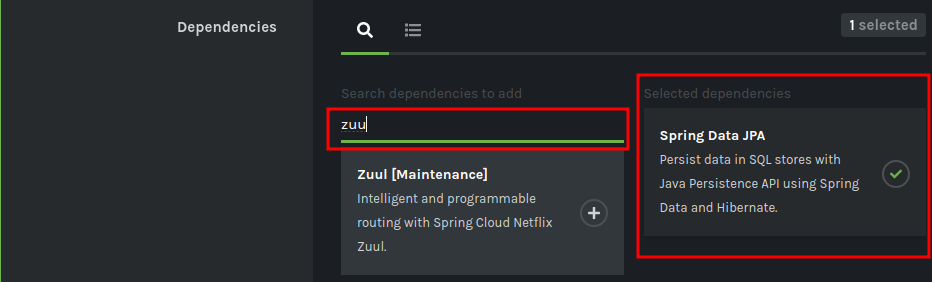
\includegraphics[width=\pictureWidth cm]{Bilder/Kapitel_4/init_dep.png}
\caption{Wahl der Abhängigkeiten in \textit{Spring Initializr}\label{fig:init_dep}}
\end{figure}

\end{enumerate}

\subsection*{Abhängigkeiten}
\label{sec:dependencies}

Da der Prototyp der neuen Hochschul-\ac{App} bereits eine breite Auswahl an Funktionen unterstützen soll und dabei auch ständig Erweiterbar und leicht zu pflegen bleiben muss, wurden in das Projekt eine Auswahl an Abhängigkeiten eingefügt. Diese werden hier nun kurz aufgelistet.

\subsubsection*{Spring Web}
Die Sammlung der vom \textit{Spring}-Framework benötigten Abhängigkeiten ist im Projekt in einer Dependency zusammengefasst. Die benötigte \textit{Maven} Dependency sieht wie folgt aus:
\begin{lstlisting}[caption={\textit{Spring Web} Dependency}]
<dependency>
    <groupId>org.springframework.boot</groupId>
    <artifactId>spring-boot-starter-web</artifactId>
</dependency>
\end{lstlisting}

\subsubsection*{JPA}
Für die Einbindung der Datenbanken wird in allen Services \ac{JPA} verwendet. \textit{Spring Boot} verwendet hierzu die \ac{JPA} Implementierung \textit{Hibernate}. Die benötigte \textit{Maven} Dependency sieht wie folgt aus:
\begin{lstlisting}[caption={Spring Data JPA Dependency}]
<dependency>
    <groupId>org.springframework.boot</groupId>
    <artifactId>spring-boot-starter-data-jpa</artifactId>
</dependency>
\end{lstlisting}

\subsubsection*{H2} 
\textit{H2} ist eine \textit{In.Memory} Datenbank, welche im Prototypen der Hochschul-\ac{App} als Testdatenbank genutzt wird, um nicht eine dauerhafte Verbindung zum Datenbank Server der Hochschule aufbauen zu müssen. Die benötigte \textit{Maven} Dependency sieht wie folgt aus:
\begin{lstlisting}[caption={H2 Dependency}]
<dependency>
    <groupId>com.h2database</groupId>
    <artifactId>h2</artifactId>
    <scope>runtime</scope>
</dependency>
\end{lstlisting}

\subsubsection*{MySQL \ac{JDBC} Dependency}
Um auf den Datenbank Server der Hochschule zuzugreifen benötigt das Projekt einen \ac{JDBC}. Da auf dem Server eine \textit{MySQL} Datenbank installiert ist wurde ein \textit{MySQL}-\ac{JDBC} eingebunden. Die benötigte \textit{Maven} Dependency für die Version des \textit{MySQL}-Servers sieht wie folgt aus:
\begin{lstlisting}[caption={\textit{MySQL} JDBC}]
<dependency>
    <groupId>mysql</groupId>
    <artifactId>mysql-connector-java</artifactId>
    <version>5.1.6</version>
</dependency>
\end{lstlisting}

\subsubsection*{DevTools}
Das in Kapitel \ref{sec:hot_deploy} erwähnte Entwicklertool \textit{Hot Deployment} benötigt ebenfalls eine Abhängigkeit, um in \textit{Spring Boot} zu funktionieren. Die benötigte \textit{Maven} Dependency sieht wie folgt aus:
\begin{lstlisting}[caption={\textit{Spring} DevTool Dependency}]
<dependency>
    <groupId>org.springframework.boot</groupId>
    <artifactId>spring-boot-devtools</artifactId>
    <scope>runtime</scope>
    <optional>true</optional>
</dependency>
\end{lstlisting}


\subsubsection*{Hypermedia}
Die \ac{HATEOAS} Funktion wurde bereits  ausführlich in der parallel zu dieser Arbeit entwickelten Bachelorarbeit erläutert\autocite[][]{dnba}. Leider konnte diese Funktion nicht in den Umfang der fertiggestellten Funktionen aufgenommen werden. Genaueres dazu wird in Kapitel \ref{sec:probleme} angesprochen. Die Dependency wird eingefügt, jedoch auskommentiert, da das Projekt ohne die Nutzung der Abhängigkeit nicht korrekt funktioniert. Die benötigte \textit{Maven} Dependency sieht wie folgt aus:
\begin{lstlisting}[caption={\ac{HATEOAS} Dependency},commentstyle=\color{red}]
<!-- UNCOMMENT ONLY IF THIS TECHNOLOGY IS IMPLEMENTED, OTHERWISE NO BUILD-->
<!--dependency>
    <groupId>org.springframework.boot</groupId>
    <artifactId>spring-boot-starter-hateoas</artifactId>
</dependency-->
\end{lstlisting}

\subsubsection*{\textit{Eureka} Client}
Die Service Discovery des Gesamtprojektes baut auf der von Netflix entwickelten \textit{Eureka}-Bibliothek auf. Um sich auf einem \textit{Eureka} Server registrieren zu können muss ein Service ebenfalls ein \textit{Eureka} Client sein. Die benötigte \textit{Maven} Dependency sieht wie folgt aus:
\begin{lstlisting}[caption={\textit{Eureka} Service Discovery Client Dependency}]
<dependency>
    <groupId>org.springframework.cloud</groupId>
    <artifactId>
        spring-cloud-starter-netflix-eureka-client
    </artifactId>
</dependency>
\end{lstlisting}

\newpage
\subsubsection*{Lombok}
Die Verwendung von \textit{Lombok} wurde in Kapitel \ref{sec:lombok} bereits ausführlich erläutert. Die benötigte \textit{Maven} Dependency sieht wie folgt aus:
\begin{lstlisting}[caption={Lombok Dependency}]
<dependency>
    <groupId>org.projectlombok</groupId>
    <artifactId>lombok</artifactId>
    <optional>true</optional>
</dependency>
\end{lstlisting}

\subsubsection*{Swagger}
Zur automatischen Generierung der Endpunkt-Dokumentation wird \textit{Spring-Fox Swagger} genutzt. Durch \textit{Swagger} kann man \ac{REST}ful Services einheitlich dokumentieren. Durch eine einfache, Menschen-lesbare Sprache, die auf \textit{yaml} beruht, können sowohl Entwickler, als auch Maschinen die Definition verstehen.
\begin{lstlisting}[caption={\textit{Swagger} Dependency}]
<dependency>
    <groupId>io.springfox</groupId>
    <artifactId>springfox-swagger2</artifactId>
    <version>2.9.2</version>
</dependency>
\end{lstlisting}
Aus der generierten Dokumentation lässt sich ebenfalls eine automatisierte Nutzeroberfläche generieren, welche zum Testen der Endpunkte genutzt werden kann. Diese Website wird automatisch in allen Services deployed und hilft den Nutzern, die Endpunkt-Dokumentation durch eine leicht verständliche Visualisierung besser zu verstehen.
\begin{lstlisting}[caption={\textit{Swagger-UI} Dependency}]
<dependency>
    <groupId>io.springfox</groupId>
    <artifactId>springfox-swagger-ui</artifactId>
    <version>2.9.2</version>
</dependency>
\end{lstlisting}

\subsubsection*{Test dependencies}
Zum testen der einzelnen Services werden mehrere Test-Frameworks benötigt. Dazu gehören unter anderem JUnit, aber auch die von \textit{Spring} eigens entwickelten Frameworks zum mocken verschiedener Abhängigkeiten. Zum Testen der Anwendung wird in Kapitel \ref{sec:test} mehr geschrieben. Die benötigten \textit{Maven} Dependencies sehen wie folgt aus:
\begin{lstlisting}[caption={Test Dependencies}]
<dependency>
    <groupId>org.springframework.boot</groupId>
    <artifactId>spring-boot-starter-test</artifactId>
    <scope>test</scope>
    <exclusions>
        <exclusion>
                <groupId>org.junit.vintage</groupId>
            <artifactId>junit-vintage-engine</artifactId>
        </exclusion>
    </exclusions>
</dependency>

<dependency>
    <groupId>org.assertj</groupId>
    <artifactId>assertj-core</artifactId>
    <scope>test</scope>
</dependency>
\end{lstlisting}

\subsubsection*{Eureka Server}
Damit der Discovery Service die Registrierungen der Services dynamisch konfigurieren und verwalten kann, muss der Discovery Service als Eureka Server fungieren. Die dafür benötigte Maven Dependency sieht wie folgt aus:
\begin{lstlisting}[caption={Eureka Server Dependencies}]
<dependency>
    <groupId>org.springframework.cloud</groupId>
    <artifactId>
        spring-cloud-starter-netflix-eureka-server
    </artifactId>
</dependency>
\end{lstlisting}

\subsubsection*{Spring Cloud Gateway}
Um die Requests der Benutzer an die registrierten Services weiterleiten zu können, benötigt der Proxy Service die Adressen der registrierten Services. Dies wird durch die Konfiguration des Spring Cloud Gateways durchgeführt. Die dafür benötigte Maven Dependency für den Proxy Service sieht wie folgt aus: 
\begin{lstlisting}[caption={Spring Cloud Gateway Dependencies}]
<dependency>
    <groupId>org.springframework.cloud</groupId>
    <artifactId>spring-cloud-starter-gateway</artifactId>
</dependency>
\end{lstlisting}

\subsubsection*{Firebase Cloud Messaging}
Um die Push Benachrichtigungen über den Notification Service versenden zu können wird die offizielle \textit{Firebase Admid \ac{SDK}} eingebunden. Dies wurde bereits in Kapitel \ref{sec:notification} erwähnt. Die dafür benötigte Maven Dependency für den Notification Service sieht wie folgt aus: 
\begin{lstlisting}[caption={FCM Dependencies}]
<dependency>
    <groupId>com.google.firebase</groupId>
    <artifactId>firebase-admin</artifactId>
    <version>6.11.0</version>
</dependency>
\end{lstlisting}

\subsection*{Wichtige Annotations}
\label{sec:annotations}

Eine der Eigenschaften, die \textit{Spring Boot} auszeichnet, ist seine Fähigkeit, komplexe Zusammenhänge und Techniken, die ihren Ursprung im Java \ac{EE} Umfeld haben, zu abstrahieren und dem Nutzer eine gut verständliche, leicht lesbare Lösung zu bieten. Das Konzept, auf das \textit{Spring Boot} dabei verstärkt setzt sind aussagekräftige Annotations. Bereits bei der Initialisierung eines Services müssen einige Voreinstellungen durch Annotations durchgeführt werden. Diese werden im Zusammenhang mit ihrer Positionierung im folgenden kurz erläutert.

\subsubsection*{Anwendungseinstieg}

Die Wurzel eines jeden \textit{Spring Boot} Programms ist die Klasse, welche die \textsc{main}-Methode als Einstieg definiert. Diese Klasse wird in allen \textit{Spring} Anwendungen mit der Annotation \textsc{@SpringBootApplication} gekennzeichnet. Zusätzlich wird diese Klasse in den funktionalen Microservices des Prototypen der neuen Hochschul-\ac{App} mit der Annotation \textsc{@EnableEurekaClient} gekennzeichnet. Das bewirkt, dass diese Services sich bei dem in den Konfigurationen definierten \textit{Eureka}-Server als Clients registrieren.\\
\linebreak
Einige Services benötigen ebenfalls Jobs, welche in bestimmten Zeitintervallen ihre Funktionalitäten ausführen. Diese Jobs nennt man \textit{Scheduled Jobs}. Beispiele hierfür sind der \textit{Timetable-Service}, welcher ständig prüft, ob in seiner Datenquelle neue Kurse oder Änderungen eingetragen wurden und der \textit{Mensa-Service}, welcher in festen Abständen die neuen Speisepläne aus seiner Datenquelle zieht. \\
\linebreak
Die Einstiegsklasse sieht damit in der Regel folgendermaßen aus:

\begin{lstlisting}[caption={Spring Application Klasse}]
@EnableEurekaClient
@SpringBootApplication
@EnableScheduling
public class TestServiceApplication{
    public static void main(String[] args) {
        SpringApplication.run(TestServiceApplication.class, args);
    }
} 
\end{lstlisting}

\subsubsection*{Controller}

Die Klassen, die die Endpunkte verwalten und die Anfragen an die Services bearbeiten heißen in \textit{Spring} \textsc{Controller}. Um der Autokonfiguration von \textit{Spring Boot} zu symbolisieren, dass eine Klasse ein Controller ist, benötigt sie die Annotation \textsc{@RestController}. Damit der Service den \ac{URL}-Pfad einer Anfrage zu einer solchen Klasse zuordnen kann, wird die Annotation \textsc{@RequestMapping([PFAD])} benötigt. Diese Klassen benötigen in der Regel noch Property Objekte, an die sie die eigentliche Bearbeitung der Anfrage delegieren können. Diese Klassen befinden sich in der Service-Schicht, enthalten die Business Logik und heißen dementsprechend Service Klassen. Damit \textit{Spring Boot} diese Objekte als Java-Bean zur per Dependency Injection zur Verfügung stellen kann, müssen die privaten Instanzen mit der Annotation \textsc{@Autowired} versehen werden. Eine entsprechende Controller Klasse sieht dann folgendermaßen aus:

\newpage
\begin{lstlisting}[caption={Spring Controller Klasse}]
@RestController
@RequestMapping("/test")
public class TestController {

    private final Service service;

    @Autowired
    public TestController(Service service){
        this.service = service;
    }
} 
\end{lstlisting}

\subsubsection*{Service}

Die Business Logik der \textit{Spring}-Anwendung liegt in der Regel in sogenannten \textit{Service}-Klassen. Das ist auch in sämtlichen Microservices des Prototypen der neuen Hochschul-\ac{App} der Fall. Damit das \textit{Spring}-Framework diese Klassen erkennt und als Beans für die Controller zur Verfügung stellen kann müssen sie mit der Annotation \textsc{@Service} markiert werden. Des weiteren benötigen diese Klassen, ähnlich wie die Controller Klasse, eine Instanz der Klasse aus der unter der Service-Schicht liegenden Persistenz-Klasse. Im Falle der Hochschul-\c{App} wird \ac{JPA} verwendet, weshalb lediglich ein Verweis auf die benötigten \acp{DAO} der Entity Klassen injiziert werden muss. Das geschieht wiederum mit der Annotation \textsc{@Autowired}. Die Service Klassen sehen in den Hochschul-\ac{App} Microservices in der Regel wie folgt aus:

\begin{lstlisting}[caption={Spring Service Klasse}]
@Service
public class TestServiceImpl implements TestService{

    private final TestDAO dao;

    @Autowired
    public TestServiceImpl(TestDAO dao){
        this.dao = dao;
    }
} 
\end{lstlisting}

\subsubsection*{JPA}

Die Tabellen, die in den Datenbanken der neuen Hochschul-Anwendung benötigt werden, werden bei der Verwendung von \ac{JPA} als \ac{POJO}-Klassen definiert, die man auch als \textit{Business Entity} oder \textit{DataObject} bezeichnet. Passend dazu müssen solche Klassen, um von \ac{JPA} als Tabelle kannt zu werden, mit der Annotation \textsc{@Entity} markiert werden. Die Annotation \textsc{@Table(name=[Table_Name])} legt dabei den Namen der Tabelle fest, die \ac{JPA} in der Datenbank anlegen - oder falls schon vorhanden - verwenden soll. Jede Klasse, die als \textit{Entity} markiert wurde, muss ein Klassenattribut besitzen, welches mit \textsc{@Id} annotiert wird. Alle Attribute der Klasse können zudem mit \textsc{@Column(name=[Column_Name])} markiert werden, was den Spaltennamen des Attributs in der Datenbanktabelle festlegt. Des weiteren können komplexere Beziehungen mit anderen Annotations festgelegt werden. Diese können in der Dokumentation der \ac{JPA} Schnittstelle nachgelesen werden\autocite[][]{jpa_oracle}. Solche Entity Klassen können wie folgt aussehen:

\begin{lstlisting}[caption={Spring Entity Klasse}]
@Entity
@Table(name="T_TEST_ENTITY")
@Getter
@Setter
@NoArgsConstructor
@AllArgsConstructor
public class TestEntity{

    @Id
    @Column(name="TEST_ID")
    private Long id;

    @Column(name="VALUE")
    private String value;
    
} 
\end{lstlisting}

\subsubsection*{Sonstige}

Wie bereits erwähnt zeichnet sich das \textit{Spring}-Framework besonders durch seine starke Abstraktion komplexer Zusammenhänge aus. Dabei kann man zwar alle Zusammenhänge klassisch über Konfigurationsdateien - in der Regel \ac{XML} oder Property-Files - definieren, jedoch liegt die Stärke des Frameworks besonders in der annotationsbasierten Konfiguration. Zusätzliche Features, wie das \textit{Swagger}-Framework, können in der Applikationsklasse per Annotation aktiviert werden. Ein Beispiel hierfür ist die erwähnte \textit{Swagger} Annotation \textsc{@EnableSwagger2}. Weitere funktionstragende Klassen, welche als Java Bean in die Applikation eingebunden werden sollen, werden ebenfalls annotiert. Beispiele hierfür sind \textsc{@Component} und \textsc{@Configuration}. 

\subsection*{Ressourcen}
\label{sec:resources}

In \textit{Spring Boot} gibt es, wie bereits erwähnt, mehrere Möglichkeiten, die Anwendung zu konfigurieren. Dabei wird im Prototypen der neuen Hochschul-\ac{App} großenteils die annotationsbasierte Konfiguration verwendet. Dennoch gibt es einige Einstellungen, welche sich am einfachsten durch sogenannte Property Files einrichten lassen. Diese müssen für jeden Microservice einzeln angelegt werden und liegen in den Ressourcen der Anwendung. Sie werden standardmäßig \textit{application.properties} benannt und enthalten in den Microservices der Hochschul-Anwendung mindestens folgende Einstellungen:

\begin{itemize}
\item \textbf{Name}\\
Unter dieser Eigenschaft wird der Name des Services festgelegt. Dieser ist vor allem bei der Registrierung beim Eureka Server und beim \ac{API}-Gateway wichtig. Der vollständige Name der Property lautet \textsc{spring.application.name}.
\item \textbf{Port}\\
Diese Eigenschaft legt den Port fest, auf dem der embedded \textit{Tomcat}-Server, der den Microservice hostet, hören soll. Der vollständige Name der Property lautet \textsc{server.port}.
\item \textbf{Eureka-Konfiguration}\\
Für die Registrierung des Eureka Clients beim Server müssen einige Einstellungen definiert werden. Die wichtigsten werden im Beispiel \ref{code:properties} gezeigt.
\item \textbf{Log}\\
Bei einer Anwendung kann es oft sinnvll sein, wichtige Ereignisse zu loggen. Damit diese im Nachhinein abgespeichert und ausgewertet werden können, gibt es dazu eine Sammlung von Properties. Die wichtigsten werden im Beispiel \ref{code:properties} gezeigt.
\item \textbf{Datenbankverbindung}\\
Um eine Verbindung zu den Datenbank Servern aufbauen zu können, benötigt \textit{Spring Boot} eine Reihe von Informationen. Diese beschreiben in der Regel die logische Adresse des Servers, den Nutzernamen, den die Anwendung als Datenbanknutzer zugewiesen bekommen hat und das passende Passwort für diese Verbindung. Des weiteren benötigt die Anwendung dann noch Details zum Namen der genauen Datenbank, mit der sie sich verbinden soll, die Art der Installation des Servers und eventuell auch Informationen dazu, wie sich \ac{JPA} bei einer Verbindung mit dem Datenbank Server verhalten soll. Da es hierbei zahlreiche Einstellungsmöglichkeiten gibt und in einer Properties-Datei mehrere Datenbanken eingebunden werden können, wird im Beispiel \ref{code:properties} exemplarisch die Datenbank des \textit{Lx-Lehre} Servers eingebuunden. Hierbei wurden sensible Daten jedoch anonymisiert. 
\end{itemize}

Das folgende Beispiel orientiert sich an den Einstellungen in den \textit{application.properties} des \textit{Timetable}-Microservices. Hierbei wurden aus Gründen des Leseflusses allerdings nicht alle Properties aufgenommen. Die sensiblen und sicherheitstechnisch relevanten Attribute wurden anonymisiert.

\begin{lstlisting}[caption={Typische \textit{application.properties} Datei}, label={code:properties}]
spring.application.name=timetable-service
server.port=8080

eureka.client.register-with-eureka=true
eureka.client.fetchRegistry=true
eureka.client.serviceUrl.defaultZone=
	http://localhost:8081/eureka/

logging.level.org.springframework.web=WARN
logging.level.org.hibernate=ERROR
logging.file.name = ./logs/timetable-service.log

spring.datasource.lx-lehre.jdbc-url=
	jdbc:mysql://localhost:60012/default_database
spring.datasource.lx-lehre.username=default_user
spring.datasource.lx-lehre.password=5AF3_PA55W0RD
spring.datasource.lx-lehre.driver-class-name=
	com.mysql.jdbc.Driver
spring.datasource.lx-lehre.jpa.hibernate.hbm2ddl.auto=none
spring.datasource.lx-lehre.jpa.show-sql=true
\end{lstlisting}

\section{Spring Cloud Gateway}

Das Framework \textit{Spring Cloud Gateway} basiert auf den Frameworks \textit{Spring 5}, \textit{Project Reactor} und \textit{Spring Boot 2.0} und bietet eine breite Auswahl an Einstellungsmöglichkeiten. Es können Filter und Routen für spezielle Anfragen definiert werden, Discovery Clients eingebunden werden, Verschlüsselungen konfiguriert und \ac{CORS}-Einstellungen definiert werden. Von all diesen Funktionen ist für den Prototypen der neuen Hochschul-\ac{App} jedoch nur die Konfiguration von \ac{CORS} und Routen zu den Microservices relevant.

\subsection*{Routen Konfiguration}

Um die Anfragen der Clients an die richtigen Microserviecs weiterleiten zu können, müssen für jeden Client Routen definiert werden. Hierfür bietet das \textit{Spring Cloud Gateway}-Framework zwei Möglichkeiten.\\
\linebreak
\textbf{Möglichkeit 1}: Statische Routen Definition über Property- oder \ac{YAML}-Files. 

\begin{lstlisting}[caption={Gateway \textit{application.yml} Datei}, label={code:ymlgateway}]
spring:
  cloud:
    gateway:
      routes:
      - id: mensa-service
        uri: lb://MENSA-SERVICE
     	- Path=/api/mensa-service/v1/**
        filters:
        - RewritePath=/api/mensa-service/v1/(?<resource>.*), /${resource}
\end{lstlisting}

Die se Möglickeit ist vor allem sinnvoll, wenn nur wenige Routen definiert werden müssen, die sich nicht ändern. Für komplexere Konfigurationen eignet sie sich jedoch nicht. Deshalb wurde im Prototypen der Hochschul-\ac{App} die sogenannte \textit{Fluent-\ac{API}} verwendet.\\
\linebreak
\textbf{Möglichkeit 2}: Dynamische Routen-Definition (Fluent-\ac{API}) über die Einbindung eines Beans vom Typ \textsc{RouteLocator}. Die Einbindung dieser Bean kann in der \textit{Spring} Application Klasse erfolgen, da es sich aber um eine Konfiguration handelt wurde der \textit{Best Practice} Vorsatz einer \textsc{@Configuration}-Klasse genutzt.

\begin{lstlisting}[caption={Gateway Routen Konfiguration Klasse}, label={code:configgateway}]
@Configuration
public class RouteConfig {

    @Bean
    public RouteLocator proxyRoutes(RouteLocatorBuilder routeLocatorBuilder){
        return routeLocatorBuilder.routes()
            .route(route -> route.path("/api/mensa-service/v1/**")
                .filters(filter -> filter
                    .rewritePath(
                     "/api/mensa-service/v1/(?<resource>.*)", 
                     "/${resource}"))
                .uri("lb://MENSA-SERVICE")
                .id("mensa-service"))
            .build();
\end{lstlisting}

Hierbei zu beachten ist die eingebundene \ac{URL} in den Codebeispielen \ref{code:ymlgateway} und \ref{code:configgateway}. Hier werden die Vorteile des Eureka Servers voll ausgenutzt. Hierfür wird in der \textit{application-properties} lediglich der Pfad zum Eureka Server eingetragen, worauf das \textit{Spring Cloud Gateway}-Framework die benötigten Servicepfade selbstständig beziehen kann.

\subsection*{Cross-Origin-Filter Konfiguration}

Da die \ac{REST}-Schnittstelle und die Clients dieser \ac{API} meist auf unterschiedlichen Quellen laufen und viele Clients ihre Anfragen über einen Browser durch \ac{CORS} realisieren, scheitern jegliche Anfragen in der Regel an mangelnden Einstellungen zur Sicherheit bei der Nutzung mit \ac{CORS}. Da diese anfällig für Angriffe sind, blockieren die gängigen Browser solche Anfragen in der Regel. Deshalb muss das \ac{CORS} im \ac{API}-Gateway uzerst konfiguriert werden, dies erfolgt wie auch bei den Routen entweder über die Poperties- oder \ac{YAML}-Files oder über die Bereitstellung von Configuration-Beans. Die bereitgestellte BEan muss zusätzlich zur \textsc{@Configuration} Annotation noch mit \textsc{@EnableWebFlux} markiert werden. \textit{WebFlux} ist ein Framework von \textit{Spring} und bietet eine reaktive Programmierunterstützung für Webanwendungen.

\newpage
\begin{lstlisting}[caption={CORS-Filter Konfigurationsklasse}, label={code:cors}]
@Configuration
@EnableWebFlux
public class CORSFilterConfig implements WebFluxConfigurer {

    @Bean
    public CorsWebFilter corsWebFilter() {
        CorsConfiguration corsConfiguration = new CorsConfiguration();
        corsConfiguration.addAllowedMethod("*");
        corsConfiguration.addAllowedOrigin("*");
        corsConfiguration.addAllowedHeader("*");
        corsConfiguration.setAllowCredentials(true);

        UrlBasedCorsConfigurationSource urlBasedCorsConfigurationSource = new UrlBasedCorsConfigurationSource();
        urlBasedCorsConfigurationSource
            .registerCorsConfiguration("/**", corsConfiguration);

        return new CorsWebFilter(urlBasedCorsConfigurationSource);
}

    @Override
    public void addCorsMappings(CorsRegistry corsRegistry){
        corsRegistry.addMapping("/**")
                .allowedMethods("*")
                .allowedOrigins("*")
                .allowedHeaders("*")
                .allowCredentials(true);
    }
}
\end{lstlisting}

\section{Eureka}

Um die bereits erwähnten Vorteile der Registry und des Discovery Services aus Kapitel \ref{sec:registryanddiscovery} nutzen zu können, müssen die Eureka Clients und die Eureka Server zunächst konfiguriert werden. Die Integration der Abhängigkeiten wurde bereits in Kapitel \ref{sec:dependencies} beschrieben und die grundlegenden Konfigurationen des Eureka Clients in Kapitel \ref{sec:annotations} und \ref{sec:resources}. Dennoch sollen diese Einstellungen nochmals kurz beleuchtet werden.

\subsection*{Eureka Client}

Im folgenden werden die wichtigsten Einstellungen für die Registrierung beim Eureka-Server in der \textit{application.properties}-Datei genauer erläutert. Der Name des Services spielt eine wichtige Rolle, dieser wird beim Eureka Server als Identifikation verwendet.
\begin{lstlisting}[caption={Spring Name in \textit{application.properties} Datei}, label={code:name}]
spring.application.name=eureka-client-service-id
\end{lstlisting}
Wird ein weiterer Eureka Client mit dem selben Namen definiert, so erkennt der Eureka Server, dass es sich bei den beiden Services um eine Duplizierung handelt und übernimmt das Load Balancing zwischen diesen. Die weiteren Properties sollen nochmals genauer erläutert werden.

\begin{lstlisting}[caption={Eureka Client Einstellungen aus \textit{application.properties} Datei}, label={code:eurekaclient}]
eureka.client.register-with-eureka=true
eureka.client.fetchRegistry=true
eureka.client.serviceUrl.defaultZone=
	http://localhost:8081/eureka/
\end{lstlisting}

Das Flag \textit{register-with-eureka} aktiviert die Registrierung des Clients mit Server. Durch \textit{fetchRegistry} werden die Registrations-Informationen vom Eureka Server geladen und lokal im Cache des Client abgespeichert. Diese Infomationen werden in einem festgelegten Zeitraum aktualisiert. Dieser kann durch die Einstellung \textit{registryFetchIntervalSeconds} manuell geändert werden. Das lokale cachen der Informationen bietet den Vorteil, dass die Clients weiterhin miteinander kommunizieren können, auch wenn keine Instanz einies Eureka Servers mehr verfügbar ist. Die \textit{defaultZone} beschreibt die physische Adresse des Eureka Servers.

\subsection*{Eureka Server}

Die Funktionen des Eureka Servers wurden bereits mehrmals erläutert. Deshalb sollen hier nur kurz die nötigen Konfigurationen dargestellt werden. Zuerst muss die \textsc{@SpringBootApplication}-Klasse im Hochschul-\ac{App} Discovery-Service als Eureka-Server annotiert werden. Dies kann mithilfe der \textsc{@EnableEurekaServer} Annotation durchgeführt werden.

\begin{lstlisting}[caption={Service als Eureka Server kennzeichnen}, label={code:eurekaapplication}] 
@EnableEurekaServer
@SpringBootApplication
public class DiscoveryServiceApplication {

    public static void main(String[] args) {
        SpringApplication
            .run(DiscoveryServiceApplication.class, args);
    }

}
\end{lstlisting}

Des weiteren muss die \textit{application.properties} Datei Konfiguriert werden. Hierfür wird auf das Kapitel \ref{sec:dependencies} verwiesen.\\
\linebreak
Es müssen wieder die gleichen Properties wie bei einem Eureka Client eingestellt werden, mit dem Unterschied, dass es sich hierbei um einen Eureka Server handelt und somit die Registrierung bei einem Server und das Laden von Informationen der registrierten Clients deaktiviert werden. Dies ist in diesem konkreten Anwendungsfall von Nöten, da es nur einen Eureka Server in der gesamten Anwendung gibt. Bei einer gewünschten Redundanz dessen ist eine andere Konfiguration nötig. Die \textsc{eureka.server} Einstellungen sind für die Minimierung der Startzeit des Servers nötig.

\section{API Filter}

Da bei \ac{REST}-Services üblicherweise Daten angeboten werden, die man in Form von Listen abrufen kann, bietet es sich oft an, einer Anfrage Filterkriterien anzufügen, nach denen die Liste schon auf dem Server gefiltert wird. So spart sich ein leichtgewichtiger Client die wertvollen Ressourcen, die bei solch einer Aktion nötig sind. Dies ist auch beim Prototypen der neuen Hochschul-\ac{App} der Fall. Daten wie Vorlesungen, Speisen und Stundenplanänderungen können im Ganzen vom Server abgerufen werden. Zusätzlich sind sie noch in Kategorien unterteilt, über die die Suche anhand des Ressourcenpfades verfeinert werden kann. Dennoch gibt es Attribute in diesen Daten, die nicht in eine solche Kategorie fallen. Typischerweise sind das Zeitangaben oder sehr spezielle Eigenschaften einer Ressource. Um dennoch nach diesen Attributen filtern zu können, werden solche Filter als sogenannte \textit{Queryparamter} übergeben. Diese werden der Endpunkt-\ac{URL} angefügt. Typischerweise sieht eine Anfrage mit solchen \textit{Queryparametern} wie folgt aus:

\begin{lstlisting}[caption={Typischer Anfragepfad mit Filtern}]
https://server.com/pfad?filter=wert&datumfilter=20-12-2018
\end{lstlisting}

In \textit{Spring Boot} können solche Parameter in der Endpunkt-Methode über die Annotation \textsc{@RequestParam} abgerufen werden. Die obere Methode würde dann folgendermaßen aussehen:

\begin{lstlisting}[caption={Typischer Endpunkt mit @RequestParam}]
@GetMapping("/pfad")
public Response testMethod(
        @RequestParam(name="filter", required=false) String filter, 
        @RequestParam(name="date", required=false) Date date){
	return Response
	           .ok(service.getData(filter,date))
	           .build();
}
\end{lstlisting}

Das hat den Vorteil, dass man Typ-sichere Parameter erhält, ohne sie selbst aus der Anfrage \ac{URL} auslesen zu müssen. Dennoch hat das den Nachteil, dass man Filterparameter so für jede Anfrage einzeln definieren muss. Zudem ist diese Herangehensweise sehr statisch und sehr aufwändig bei einer Änderung. Deshalb wurde für die Microservices der Hochschulanwendung eine andere Lösung implementiert.\\
\linebreak
Für die implementierte Lösung muss die Klasse \textsc{FilterTO.class} erstellt werden. Sie sieht folgendermaßen aus:

\begin{lstlisting}[caption={Aufbau des Filter Objekts}]
@Setter
@AllArgsConstructor
public class FilterTO {

    protected Map<String, String> filters;

    public Map<String, String> getFilters() {
        return Collections.unmodifiableMap(filters);
    }
}
\end{lstlisting}

Zu Beachten ist hier die verwendete \textsc{Map}, welche dafür da ist, die Namen der Filterparameter auf ihren Wert zu mappen. Die \textsc{FilterTO} Instanz wird bei jeder Anfrage in der folgenden Klasse erstellt:

\begin{lstlisting}[caption={Filterparser}]
@ControllerAdvice
public class FilterParser {

    private final HttpServletRequest request;

    @Autowired
    public TimetableFilterParser(HttpServletRequest request) {
        this.request = request;
    }

    @ModelAttribute
    public void addAttributes(Model model) {
        model.addAttribute("filter", getFilterTO());
    }

    private FilterTO getFilterTO(){
        Map<String, String> filters = new HashMap<>();
        Collections.list(request.getParameterNames())
                .forEach(name->{
                    String value = request.getParameter(name);
                    value = value
                            .replaceAll("\"", "")
                            .trim();
                    filters.put(name, value);
                });
        return new FilterTO(filters);
    }
}
\end{lstlisting}

Die Annotation \textsc{@ControllerAdvice} bewirkt, dass die Controller-Klassen, die darin explizit referenziert werden, die Möglichkeit haben, das Model der \textsc{addAttributes()}-Methode in ihren Anfragen zu injizieren. Dieses Model bekommt ein \textsc{FilterTO} Objekt, welches in seiner Map die Query Parameter enthält. Diese sind jedoch noch nicht Typ-sicher, sondern lediglich als String hinterlegt. Zudem sind in dieser Map alle Parameter, auch die, die die Controller eventuell nicht akzeptieren. Die Controller benötigen in ihren Endpunkt-Methoden folgende Definition, um auf den Filter zugreifen zu können:

\begin{lstlisting}[caption={Typischer Endpunkt mit eigener Lösung}]
@GetMapping("/pfad")
public Response testMethod(@ModelAttribute("filter") FilterTO filter){
    return Response
               .ok(service.getData(new DataFilterTO(filter)))
               .build();
}
\end{lstlisting}

Wie zu erkennen ist, ist nirgends definiert, welche Filter der Endpunkt akzeptiert. Jedoch wird an den ausführenden Service nicht das eigentliche \textsc{FilterTO} weitergegeben, sondern die Klasse \textsc{DataFilterTO.class}. Diese ist wie folgt aufgebaut:


\begin{lstlisting}[caption={Ressourcenspezifisches Filter Objekt}]
@Getter
public class DataFilterTO extends FilterTO{

    private final I18nResourceBundle I18N = new I18nResourceBundle();

    private String filter;
    private Date date;
    
    public LectureFilterTO(FilterTO filterTO){
        super(filterTO.filters);
        this.setFilter(this.filters.get("filter"));
        this.setDate(this.filters.get("date"));
    }
 
    public void setFilter(String filter){
        if(I18N.validateContent(filter))
            this.filter = filter;
    }
    
    public void setDate(String date){
        SimpleDateFormat format = new SimpleDateFormat(Constants.DATE_FORMAT);
        try{
            this.date = format.parse(date);
        }catch(ParseException pE){
            this.date = null;
        }
}
\end{lstlisting}

In dieser Klasse werden die rohen Filterdaten gesammelt und die für die angefragte Ressource erlaubten Filter in ihrem korrekten Typ extrahiert. Dies geschieht in den zu den Klassenattributen gehörenden Settern. Die Klasse \textsc{I18nResource\-Bundle.class} regelt in diesem Fall exemplarisch den Test, ob der übergebene Filter in einer der von der Anwendung unterstützten Sprachen korrekt ist. Das Datum wird ebenfalls nur dann gesetzt, wenn es im richtigen Format übergeben wurde. \textsc{Constants\-.class} ist hierbei eine globale Sammlung von Konstanten. Nach der Erstellung dieser Klasse sind nur noch Filter relevant, die die Klasse \textsc{DataFilterTO.class} auch akzeptiert. Der Service, der vom Endpunkt aufgerufen wurde, verarbeitet die Filter dann folgendermaßen:

\begin{lstlisting}[caption={Serviceschicht}]
public DataTO getData(DataFilterTO filter){
    return testDao.findAll(new FilterSpecification(filter))
               .stream()
               .map(DataDO::createTO)
               .collect(Collectors.toList());
}
\end{lstlisting}

Die Methode \textsc{findAll()} ist eine Methode des \textit{Spring Data}-Frameworks, welche Instanzen der Klasse \textsc{Specification.class} zum verfeinern der automatisch generierten Datenbankanfrage akzeptiert. Auch hier ist anzumerken, dass nach wie vor nicht kontrolliert wurde, welche Filter für diese Anfrage gesetzt wurden. Das geschieht in der folgenden Klasse:

\begin{lstlisting}[caption={Spezifikation der Filter für Datenbankanfrage}]
public class FilterSpecification implements Specification<DataDO> {

    private final DataFilterTO FILTER;
    private final Set<Specification<DataDO>> SPECIFICATIONS;
    
    public LectureFilterSpecification(LectureFilterTO filter) {
        this.FILTER = filter;
        this.SPECIFICATIONS = new HashSet<>();
    }
   
    @Override
    public Predicate toPredicate(Root<LectureDO> root, CriteriaQuery<?> criteriaQuery, CriteriaBuilder criteriaBuilder) {
        Specification<DataDO> spec = ...; /*Hier ist die Instanziierung abhaengig vom Service*/
        if(FILTER.getFilter() != null)
            spec = spec.and(this.getFilterSpecification());
        if(FILTER.getDate() != null)
            spec = spec.and(this.getDateSpecification());
        return spec.toPredicate(root, criteriaQuery, criteriaBuilder);
    }
    
    /*Implementierung der get...Specification()-Methoden unterschiedlich*/
}
\end{lstlisting}

Das Interface \textsc{testDao} des Typs \textsc{JpaRepository<DataDO, Long>, JpaSpecificationExecutor<DataDO>} liefert dann nur noch die Daten zurück, die den Filtern, die in die Datenbankanfrage durch die hinzugefügten Spezifikationen angefügt wurden, entsprechen. Diese Lösung ist zwar anfangs deutlich aufwändiger zu implementieren, als die Nutzung von \textsc{@RequestParam}, jedoch ist sie genau auf die Bedürfnisse der Schichtenarchitektur in Verbindung mit der Nutzung von \ac{JPA} angepasst und ist nach der initialen Implementierung deutlich flexibler. Neue Filter können also jederzeit hinzugefügt werden und werden so bis in die Datenbankschicht übernommen.

\section{Error Handling}

Wie bei vielen weiteren Funktionen bietet \textit{Spring Boot} ebenfalls Lösungsansätze für das Error-Handling, speziell beim Abfangen von Exceptions im Code und der Rückgabe der richtigen Status-Informationen an den aufrufenden Client. Die standardmäßig verwendeten Funktionen von \textit{Spring} sind hier jedoch nicht ausreichend, sie bieten dem Client zu viele Informationen darüber, was den Fehler ausgelöst hat. Um dies abzufangen werden im Prototypen der Hochschul-\ac{App} die Annotations \textsc{@ControllerAdvice} und \textsc{@ExceptionHandler} verwendet. Dies sieht wie folgt aus:

\newpage
\begin{lstlisting}[caption={Error Handling}]
@ControllerAdvice
public class ExceptionHandler {

    @ExceptionHandler(Throwable.class)
    public ResponseEntity<HttpReturnErrorPattern> handleUncaughtExceptions(Throwable e){
        LOGGER.warn(e.getMessage(), e);
        return handleServerException(new ServerException(e.getMessage()));
    }

    @ExceptionHandler(BaseException.class)
    public ResponseEntity<HttpReturnErrorPattern> handleServerException(BaseException e){
        LOGGER.warn(e.getMessage(), e);
        return e.toResponse();
    }
}
\end{lstlisting}

Zu erkennen ist, dass in der Klasse \textsc{ExceptionHandler} lediglich zwei Methoden vorhanden sind. Diese Methoden sind jeweils mit der Annotation \textsc{@ExceptionHandler} markiert. Diese Annotation benötigt als Parameter die Klasse des \textit{throwables}, die abgefangen werden soll. Konkret wird in der Methode \textsc{handleServerException} eine eigens entwickelte Exception abgefangen, welche sich um Informationsfluss nach außen, Internationalisierung der Antworten und Formatierung der Fehler kümmert. Die Methode \textsc{handleUncaughtExceptions} ist lediglich eine Methode, die alle Exceptions abfängt, die im Code unerwartet geworfen werden. Diese Exceptions werden anonymisiert und die Bearbeitung wird and die \textsc{handleServerException} Methode delegiert.\\
\linebreak
Diese Konfiguration ermöglicht es, alle Exceptions abzufangen und intern zu verarbeiten. Alle benötigten Infos können geloggt und entsprechend verarbeitet werden. Der Client sieht immer nur die Informationen, die er sehen darf, was mögliche Sicherheitslücken vermindert. Zudem wird nie eine Exception geworfen, die den Server zum Absturz bringt.

\section{Firebase Cloud Message}
\label{sec:notifications}

\ac{FCM} ist ein Cloud Messaging Service, der von \textit{Google} entwickelt wurde. Er stellt die Grundlage für den Notification Service dar und wird deshalb hier explizit nochmals genauer betrachtet. Für die Nutzung des \ac{FCM}-Services wird zunächst ein Google Account benötigt. Für den Prototypen der neuen Hochschul-\ac{App} wurde die E-Mail-Adresse \textit{hochschul-app-fh@gmx.de} erstellt und für den benötigten und kostenlosen Google Account verwendet. Mit dieser Mail-Adresse kann nun ein Firebase-Projekt erstellt werden. Dafür muss die Website des Services aufgerufen werden\autocite[][]{firebase_home}. Nun muss für die Konfiguration der Kommunikation zwischen dem Notification Server der Hochschul-\ac{App} und dem Firebase-Cloud Server noch ein sogenanntes \textit{Cloud Messaging}-Schlüsselpaar erstellt werden. Dieses wird danach für die \textit{Web-Push}-Zertifikate genutzt und soll den Notifikations-Client - in diesem Fall den Notification Service der Hochschul-\ac{App} - eindeutig identifizieren.

%wo kommt der PW hin? GMX OGa@89F=

\begin{figure}[H]
\centering
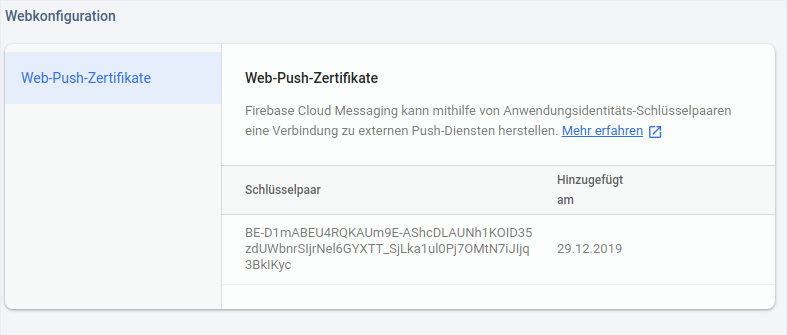
\includegraphics[width=\pictureWidth cm + 2 cm]{Bilder/Kapitel_4/firebase_webkonfiguration.png}
\caption{Firebase Webkonfiguration\label{fig:fcmwebconfig}}
\end{figure}

Für die Nutzung der \ac{FCM}-Funktionalitäten im Notification-Service der Hochschul-\ac{App} muss unter den Dienstkonten zuerst ein neuer privater Schlüssel erstellt werden. Dies sieht folgendermaßen aus:

\begin{figure}[H]
\centering
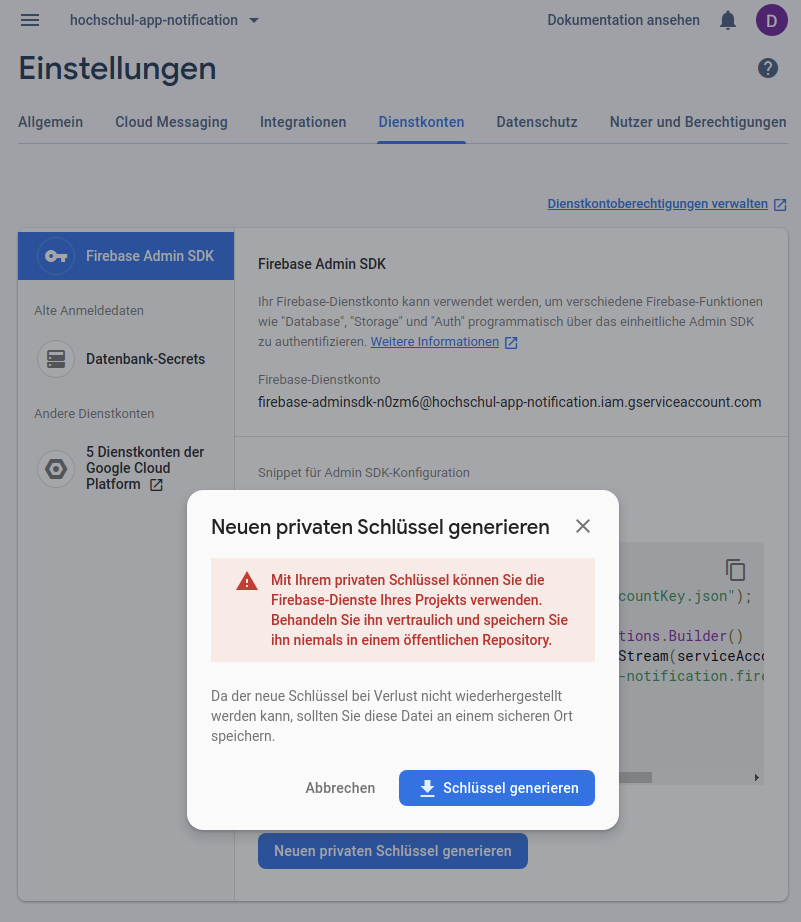
\includegraphics[width=\pictureWidth cm + 2 cm]{Bilder/Kapitel_4/fcm_privatekey.png}
\caption{Firebase Admin SDK Authentifizierung\label{fig:fcmprivatkey}}
\end{figure}

Nach diesem Schritt wird vom Firebase-Service ein \ac{JSON} generiert, welches alle relevanten Firebase-Service-Account Informationen wie Projekt-ID, Private-Key, Client-ID, Authentifikations-\ac{URL}, Tokens und die \acp{URL}  der Zertifikate enthält. Das komplette \ac{JSON}-File ist folgendermaßen aufgebaut:

\newpage
\begin{lstlisting}[caption={Firebase Service Account JSON}]
{
   "type": "service_account",
   "project_id": "hochschul-app",
   "private_key_id": "5ECUR3",
   "private_key": "-BEGIN PRIVATE KEY--END PRIVATE KEY-",
   "client_email": "firebase-adminsdk@hochschul-app.com",
   "client_id": "12345678",
   "auth_uri": "https://accounts.google.com/o/oauth2/auth",
   "token_uri": "https://oauth2.googleapis.com/token",
   "auth_provider_x509_cert_url": "https://www.google.com/certs",
   "client_x509_cert_url": "https://www.google.com/hochschul-app.com"
}
\end{lstlisting}

Dieses File muss dann im Notification-Service eingebunden werden. Dafür wird im \textit{application.properties}-File der Pfad des abgelegten \ac{JSON} definiert. Es wird dabei folgende Zeile angefügt: 

\begin{lstlisting}[caption={Firebase Service Account application.properties Datei}]
fcm.firebase-config-file=${PFAD}/firebase-adminsdk.json
}\end{lstlisting}

Im Package \textsc{config} des Source Codes des Notification-Service wird eine Klasse erstellt, die mit der Annotation \textsc{@ConfigurationProperties} markiert wurde und die Inhalte der \ac{FCM}-Properties in eine Variable schreibt.

\begin{lstlisting}[caption={Firebase Service Account Variable}]
@Setter
@Getter
@ConfigurationProperties(prefix = "fcm")
public class FcmProperties {

    private String firebaseConfigFile;

}
\end{lstlisting}

Zudem wird ein Bean der Konfigurationsklasse definiert und in den Notification Service eingebunden.

\newpage
\begin{lstlisting}[caption={Firebase Service Account Bean}]
@Configuration
@EnableConfigurationProperties(FcmProperties.class)
public class FcmPropertiesConfig {

    @Bean
    public FcmProperties fcmConfig () {
        return new FcmProperties();
    }

}
\end{lstlisting}

Mithilfe des Beans kann die Verbindung zur \ac{FCM}-Cloud dann folgendermaßen aufgebaut werden:

\begin{lstlisting}[caption={Firebase Service Account Bean}]
Path path = Paths.get(fcmPropertiesConfig.fcmConfig()
    .getFirebaseConfigFile());
InputStream inputStream = Files.newInputStream(path);
FirebaseOptions options = new FirebaseOptions
    .Builder()
    .setCredentials(
        GoogleCredentials
            .fromStream(inputStream)
    ).build();
\end{lstlisting}

Nach dem Verbindungsaufbau können im Notification Service Clients registriert sowie informiert werden. \ac{FCM} bietet zusätzlich die Möglichkeit der Erstellung von \textit{Topics}. Diese sind organisatorische Einheiten, in die Benachrichtigungen eingeteilt werden können. Somit muss sich ein Client nicht für alle Benachrichtigungen registrieren, sondern kann diese nach der Relevanz für seinen Anwendungsfall filtern.

\newpage
\begin{lstlisting}[caption={Firebase Service Account Bean}]
//build message with topic
Message message = Message.builder()
   .putAllData(messageTO.getData())
   .setTopic(topic)
   .setWebpushConfig(WebpushConfig.builder().putHeader("ttl", "300")
       .setNotification(new WebpushNotification(messageTO.getTitle(), messageTO.getBody(), icon))
       .build())
   .build();

//subscribe to topic
TopicManagementResponse response = FirebaseMessaging.getInstance()
    .subscribeToTopicAsync(
        Collections.singletonList(registrationToken), 
        topic
    ).get();

//unsubscibe from topic
TopicManagementResponse response = FirebaseMessaging.getInstance()
    .unsubscribeFromTopicAsync(
        Collections.singletonList(registrationToken), 
        topic
    ).get();

//send message
FirebaseMessaging.getInstance().sendAsync(message).get();

\end{lstlisting}